
%\renewcommand\labelitemi{\textcolor{blue}{$\bullet$}}  
\renewcommand\labelitemi{\textcolor{blue}{$\bullet$}}  
\renewcommand\normalcolor{\color{blue}}  %for titles, etc.
\renewcommand\Black{\color{black}}        %for headers, etc.
\renewcommand\labelitemii{\textcolor{DarkGreen}{$\star$}}  
\color{black}                             %for normal text


\foilhead{\textcolor{red}{C} Nebular Astrophysics}
\leftheader{C: Nebular Astrophysics}
\vpagecolor[blue]{RGBblack}                 %blue to black vertical gradient
\LogoOff
\bgclear

\vspace{-1cm}
\begin{center}
{\tt http://www.nublado.org/ }
\end{center}
\vspace{-1cm}
\begin{enumerate}
\item Atomic Processes.\\ 
Photoionization. Collisional Ionization. Recombination. Charge
Transfer. \label{item:processes}
\item Ionization Equilibrium. \\ 
Collisional Ionization in the low density limit. Photo-ionization
equilibrium.    \label{item:equi}
\item Thermal Balance.  \label{item:balance}
\item Nebular models. \\ CLOUDY. Analytical models:
pure hydrogen nebula, OTS approximation; dustry hydrogen nebula..
Problems with OTS - need for realistic radiative transfer. Escape
probabilities.  \label{item:models}
\item Temperature and density diagnostics. CELs, ORLs,
 Balmer \& Paschen discontinuities. The ORL/CEL discrepancy. \label{item:diag}
\item Detailed study: The Helix. \label{item:example}
\end{enumerate} 



\renewcommand\labelitemi{\textcolor{blue}{$\bullet$}}  
\renewcommand\normalcolor{\color{blue}}  %for titles, etc.

\foilhead{\textcolor{red}{C-\ref{item:processes}} Photoionization  }
\leftheader{C-\ref{item:processes}: Atomic processes}

\renewcommand\labelitemi{\textcolor{blue}{$\bullet$}}  
\renewcommand\Black{\color{black}}        %for headers, etc.
\renewcommand\labelitemii{\textcolor{DarkGreen}{$\star$}}  
\color{black}                             %for normal text

\LogoOff
\bgclear
\pagecolor{white}

In time-dependent perturbation theory, the rate of transition between
two states, $i\rightarrow f $, is:
\[
\frac{dP_{if}}{dt} = \frac{e^2}{h c^3 m_e^2} \sum_{\alpha = 1}^2 \int
\omega_{fi} ~\mathcal{N}_{\alpha}(\vec{k}) ~| \langle \phi_f |
e^{i\vec{k}\cdot\vec{x} } \vec{e}_{\alpha} \cdot \vec{p} | \phi_i
\rangle |^2 ~d\Omega,
\]   
where $\mathcal{N}(\vec{k})$ is the occupation number of photons in
the state corresponding to  $\vec{k}$,
with frequency  $\nu_{fi}$.

In a photoionization process the final states $f$ belong to the
continuum. The Born approximation neglects the influence of the ion on
$|\phi_f\rangle$, and for a description of the continuum we adopt a hard
box normalization, with a size  $L \rightarrow
\infty$. With  $i$ corresponding to the fundamental state of the
hydrogen atom, we obtain (Shu~I, 23),
\[
\frac{dP_{if}}{dt} \propto \omega_{fi}^{-3} \mathcal{N}(\omega),
~\text{where } \mathcal{N}(\omega) = \int d\Omega
\mathcal{N}(\vec{\omega}) .
\]


\foilhead{}

The rate of absorption of ionizing photons with frequencies in the
range $[\nu,\nu+\nu]$ is $ dN_f \frac{dP_{if}}{dt} $, where $dN_f$ is
the number of free states in the corresponding range of energies,
\[ 
dN_f = \frac{V}{2\pi^3} 4\pi~k_e^2 ~dk_e,
\]
where $\vec{k_e}$ refers to the free electron.

The cross-section of ionization is defined through
\[
P_{if} dN_f =  t~\sigma_{if}(\omega) c ~\frac{\mathcal{N}(\vec{n})}{V}
 ~4\pi n^2 dn , \text{~with } \frac{d^3\vec{n}}{V} =
\frac{d^3\omega}{(2\pi)^3 c^3}.
\]
Identifying for $\sigma(\nu)$ we get
\[
\sigma(\nu) \propto \nu^{-3}  g(\nu),
\]
where $g(\nu)$ is a gaunt factor, $g(\nu) \propto \nu^{-1/2} $, in the
Born approximation, which is valid far from the ionization edge
$\nu_\circ$. $g_\nu \approx 1 $ in the vicinity of $\nu_\circ$, where
the free-particle approximation breaks down.


\foilhead{}

\begin{center}
  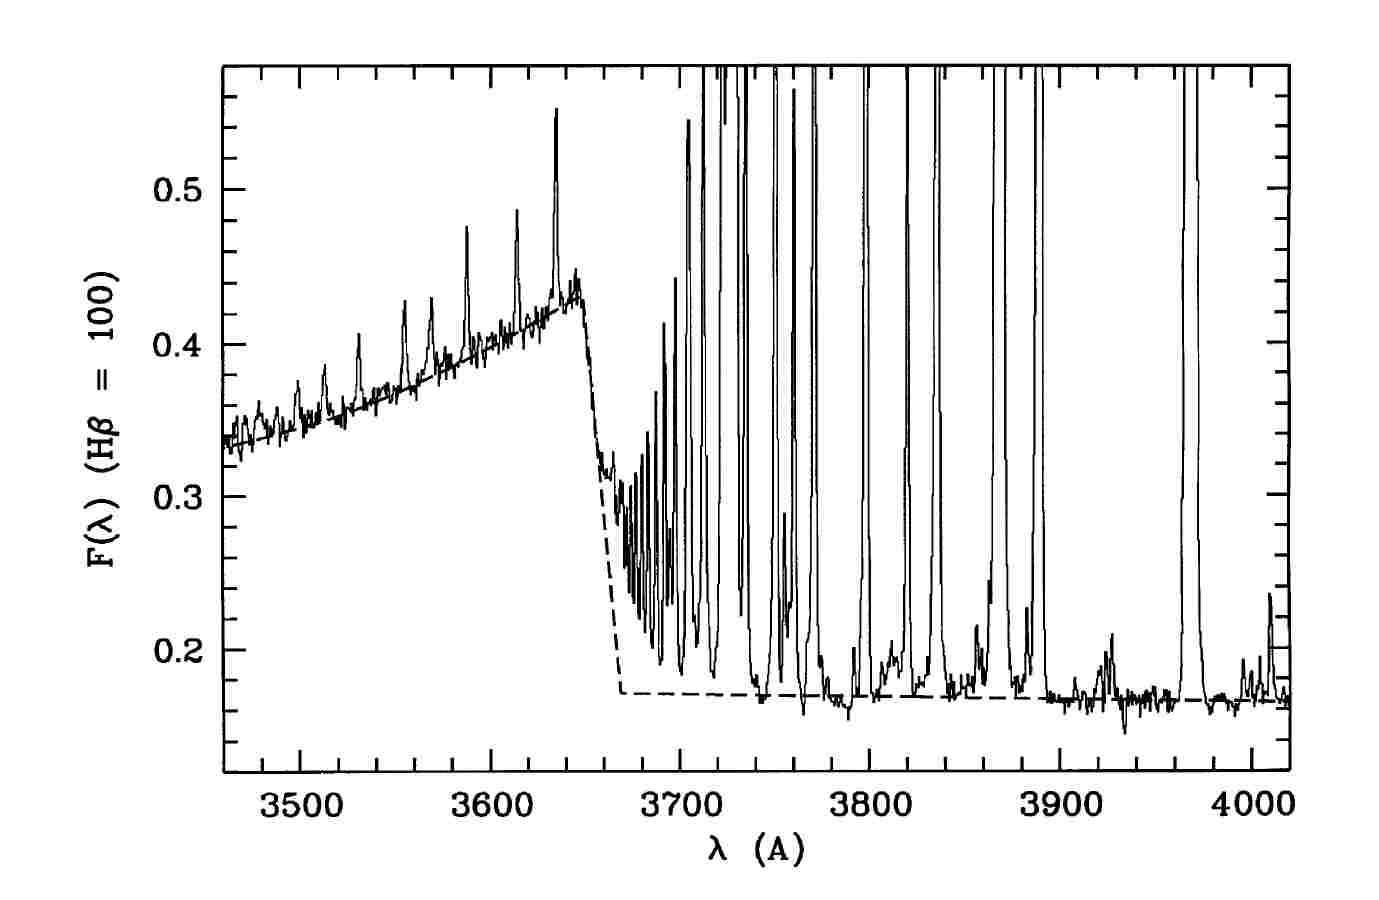
\includegraphics[width=25cm,height=!]{./C/bj_liu.jpg}
\end{center}


\foilhead{Photoionization of metals\footnote{Verner et al. 1996, ApJ, 465, 487. $1~b = 10^{-24}$~cm$^2$.}}


\begin{minipage}[t]{13cm}
  \begin{center}
    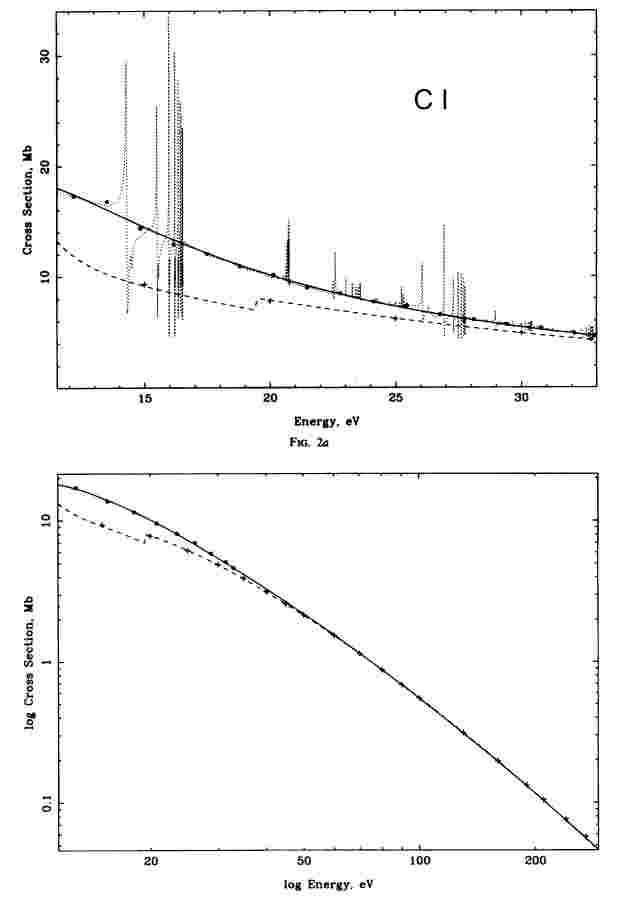
\includegraphics[width=12.5cm,height=16cm]{./C/ci_photion.jpg}
  \end{center}
\end{minipage}
%\hfill
\begin{minipage}[t]{13cm}
  \begin{center}
    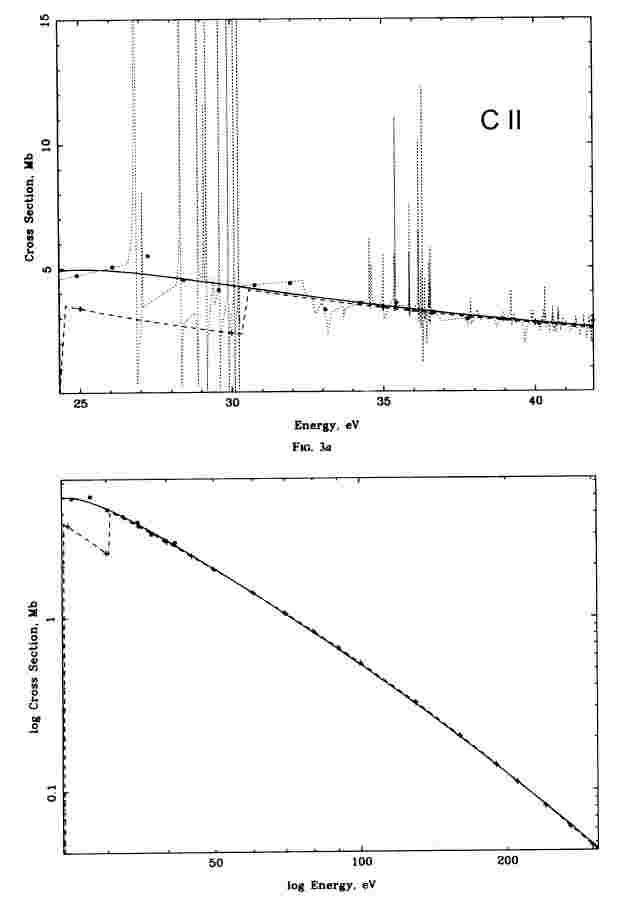
\includegraphics[width=12.5cm,height=16cm]{./C/cii_photion.jpg}
  \end{center}
\end{minipage}




\foilhead{Photoionization of metals\footnote{{\sc cloudy} manual, Hazy.}}

  \begin{center}
    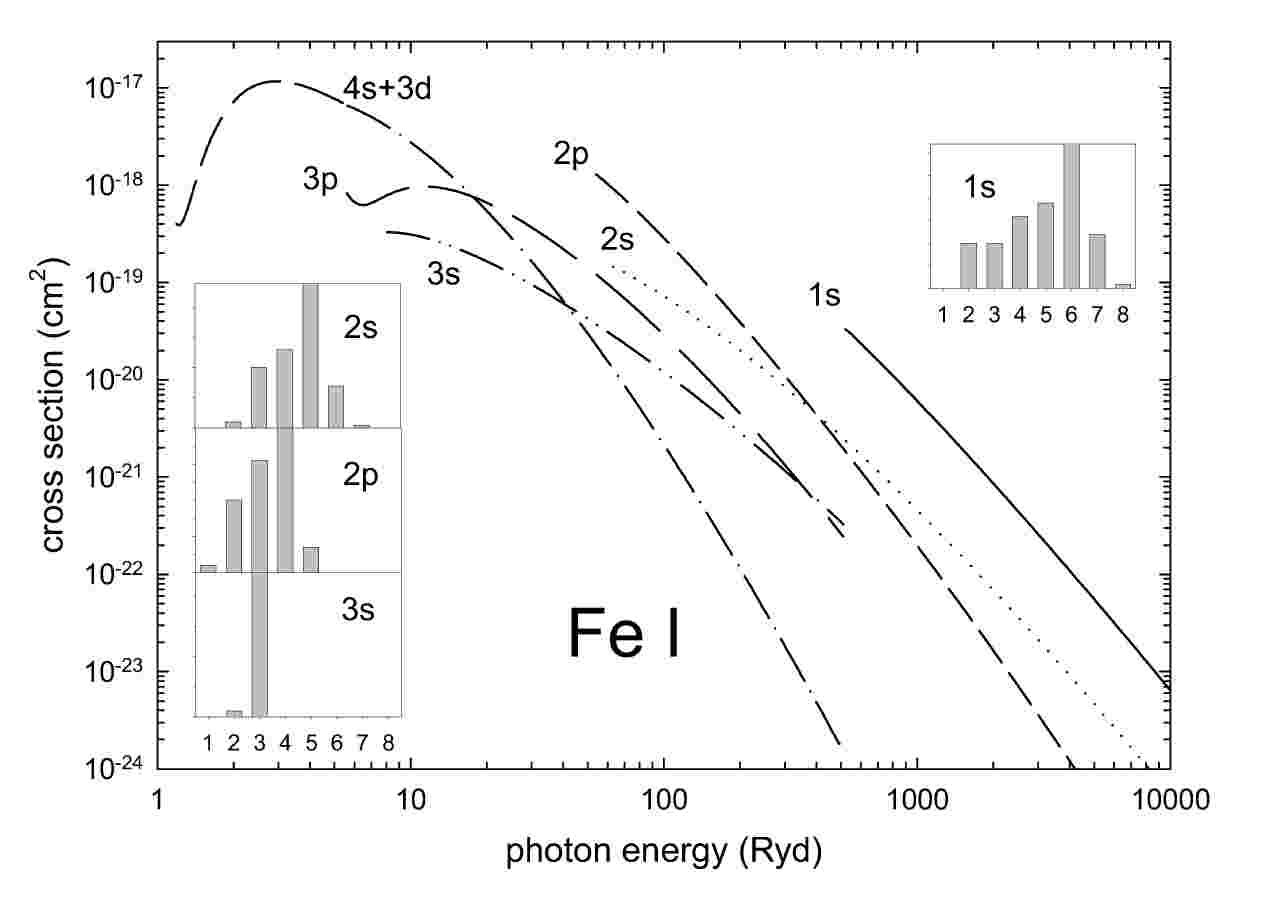
\includegraphics[width=!,height=16cm]{./C/auger_FeI.jpg}
  \end{center}



\foilhead{Collisional Ionization\footnote{Arnaud \& Rothenflug 1985, A\&AS, 60, 425; Arnaud \& Raymond, ApJ, 1992, 398, 394}}

\vspace{-2cm}
\begin{eqnarray}
\text{Direct collisional ionization: }  & \mathrm{A} + \mathrm{e} \rightarrow \mathrm{A^+} + 2~\mathrm{e}   \nonumber \\ 
\text{Excitation -- auto-ionization: }  & \mathrm{A} + \mathrm{e} \rightarrow \mathrm{A^\star} + \mathrm{e}   \nonumber  \\
                                         & \mathrm{A^{\star}}  \rightarrow \mathrm{A^+} + \mathrm{e}   \nonumber  
\end{eqnarray}
\vspace{-2cm}
\begin{center}
  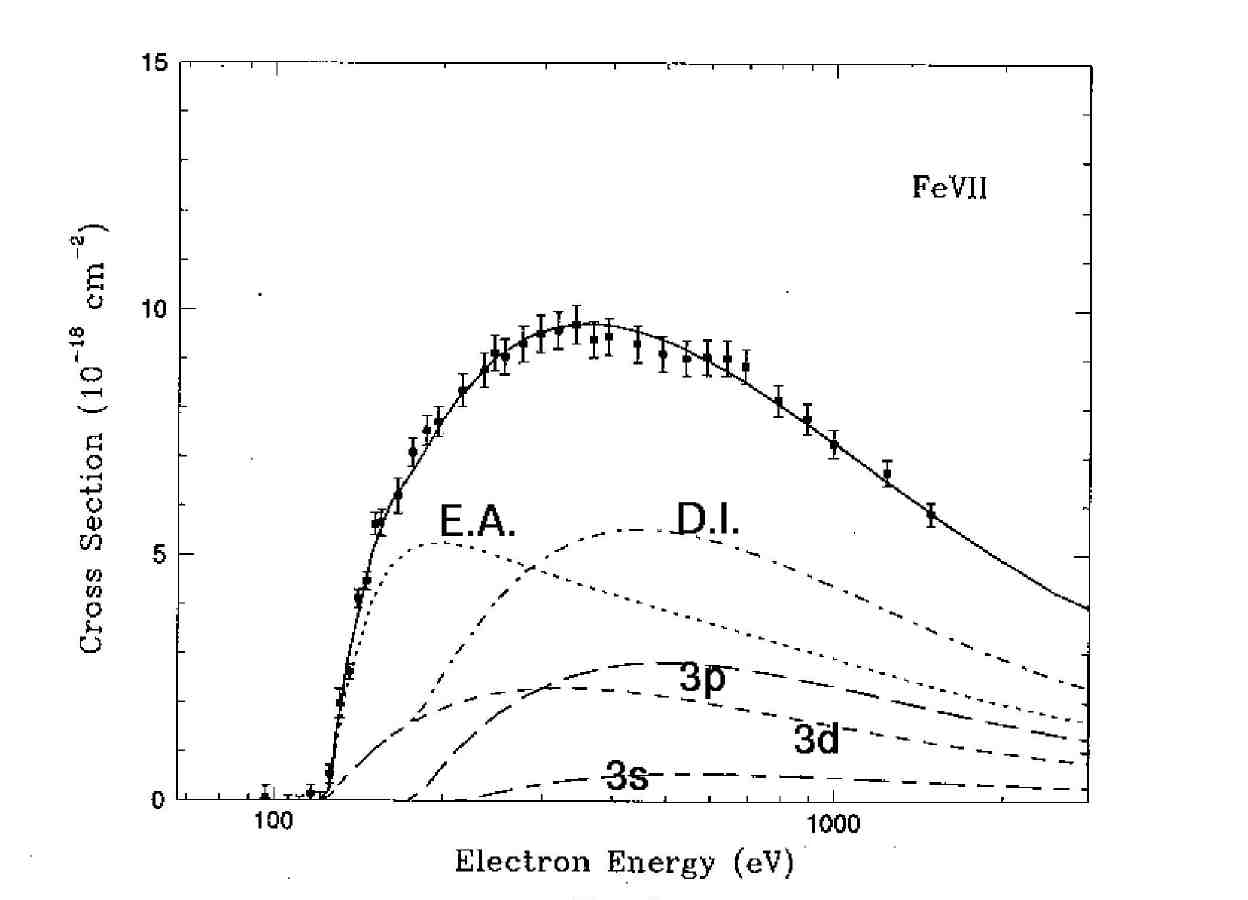
\includegraphics[width=17cm,height=!]{./C/colion_xsec_2.jpg}
  \footnote{the subshell contributions to D.I. are indicated}
\end{center}


\foilhead{Recombination}

{$\bullet$ Radiative recombination} \\

Photoionization and its inverse process, radiative recombination, are
related by the Einstein - Milne relations (e.g. Osterbrock, A1; Shu
I,75; Spitzer p104)).  The detailed balance between photon absorptions
with frequency $\nu$ and electron-ion recombinations with relative
velocity $v$ is
\[
n_\mathrm{X} ~a_\nu 4 \pi \frac{B_\nu}{h \nu} ~d\nu = n_{\mathrm{X}^+} n_e
v \sigma(v) f(v) dv~ +~ n_{\mathrm{X}^+} n_e \sigma_2(v)  B_\nu v f(v) dv,
\]
where $~\frac{1}{2} m v^2 + h \nu_T = h \nu,$ and where $f(v)$ is the
Maxwellian integrated over angles. We get (\textcolor{red}{tarea}) that
$\sigma_2 = \sigma / (2 h \nu^3 / c^2 )$, and 
\[
\sigma(v) = \frac{g}{g_{+}}   \frac{h^2  \nu^2 }{m^2 c^2 v^2} a_\nu,    
\] 
where $g$ and $g_+$ are the degeneracies of  $X$
 and  $X^+$ in their fundamental levels.


\foilhead{Recombination}

{$\bullet$ Collisional recombination} \\

Recombination through 3 body collisions 
\[
 \mathrm{A^+} + 2~\mathrm{e}  \rightarrow \mathrm{A} + \mathrm{e}, 
\]
is important in the limit of very high densities. Note high densities
is not the domain of validity of the collisional ionization
equilibria, since these assume optically thin conditions. Rather, high
densities are simply described by the law of mass-action, as in
stellar interiors. 

But another domain of validity of 3-body collisions, applicable to the
diffuse ISM, is the case of radio recombination lines of H\,{\sc i}
(e.g. H\,109$\alpha$ at 6\,cm, see Osterbrock p97).


\foilhead{Recombination}

{$\bullet$ Dielectronic recombination}

The inverse process to excitation-autoionization is the dielectronic
recombination. For example (e.g. Osterbrock 1989) consider the
recombination of C$^{++}$ in its fundamental configuration
$1s^22s^2~^1$S through the collision with a 0.41~eV electron, which
matches the energy of C$^+$ in $1s^22p3d~^2$F. Doubly excited C$^{+}$
decays following a cascade (in practice 2 photons, through
$2s2p^2~^2$D) to the ground state $1s^22s^22p~^1$P$_{1/2}$.
Generically,
\[
\mathrm{X}^{+i+1} + e \rightarrow ~^{\star}\mathrm{X}^{+i} \rightarrow \mathrm{X}^{+i} + h\nu
\]
where $^{\star}X^{+i}$ is an autoionizing state of $\mathrm{X}^{+i}$.
This is the dominant mechanism for recombination at nebular
temperatures of $10^{4}$~K and densities (Nussbaumer \& Storey, 1983,
A\&A, 126, 75). \underline{No calculations are available for elements
heavier than Ne}.

\foilhead{Charge transfer}

(Spitzer + Osterbrock) 

\[
A  + H^+  \overset{k_1}{\underset{k_2}{\rightleftharpoons}} A^+ + H
\]
{$\bullet$ relationship between the rates of forward and reverse
reactions, $k_1$ and $k_2$}


\foilhead{\foilhead{\textcolor{red}{C-\ref{item:equi}} Ionization
equilibrium - Collisional Ionization}}
\leftheader{C-\ref{item:equi}: Ionization equilibrium}


In the limit of low densities, and in the absence of external
radiation fields, the relative ionic concentrations are obtained from
detailed balance (the example is from Jordan (1969), but the
calculations from Arnaud et al. are more recent):
\[
\frac{N(X^{+(m+1)})}{N(X^{+m})} =
\frac{Q(X^{+m})}{\alpha_\mathrm{tot}(X^{+m})},
\]
where $Q$ and $\alpha_\mathrm{tot}$ are the rate coefficients for
ionization and recombinations.

\begin{center}
  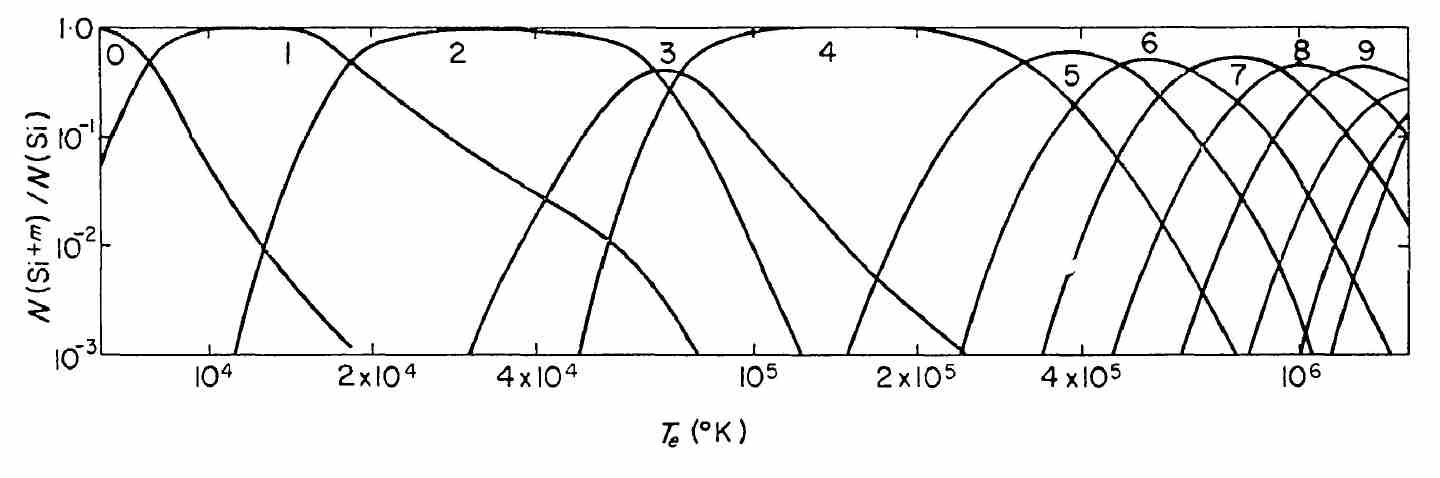
\includegraphics[width=25cm,height=!]{./C/colion_eq.jpg}
\end{center}


\foilhead{Ionization equilibrium - Photoionization}

The structure of a photoionized nebula in spherical symmetry can be
described by the ionization fraction of each element as a function of
nebular radius. For a blob of nebular material, the ionization balance
requires that the number of recombinations of ion X$^{+i+1}$ be equal 
to the number of photoionizations of  ion X$^{+i}$,
\begin{equation}
N(\mathrm{X}^{i+1}) N_{e} \alpha_{T} = {\int}d{\nu} \frac{4\pi J_{\nu}}{h\nu}
a_{\nu} N(\mathrm{X}^{i}), 
\label{eq:ionisation_balance}
\end{equation}
where $N_{e}$ is the electron density, $\alpha_{T}$ is the total
recombination coefficient, and $a_{\nu}$ is the cross-section of
photoionization, and $J_{\nu}$ is the local angular average of the
nebular specific intensity field, 
\begin{eqnarray}
J_{\nu}  & =  & \frac{1}{4~\pi}\int_{4 \pi} I_\nu d\Omega , \nonumber \\
 & = & \frac{1}{2}\int_{-1}^{+1} d\mu ~I_\nu(r,\mu), \text{~for
 spherical symmetry, with } \nonumber  \\ 
\mu &  =  & \cos \theta, \text{~where the angle   $\theta$ is measured
 relative to the radial direction.} \nonumber
\end{eqnarray}



\foilhead{\foilhead{\textcolor{red}{C-\ref{item:balance}} Thermal Balance}}
\leftheader{C-\ref{item:balance}: Thermal Balance}

(R.E. Williams, en Lecture Notes on Introductory Theoretical
Physics). 

The electron bath is the specie that thermalizes fastest in an ionized
nebula (Spitzer, Cap. II). We consider the energy balance of the electrons.

$\bullet$ {\bf \large Heating of the  electrons}.
\begin{itemize}
\item collisional de-excitation. Important in dense nebulae, and
partially compensated by collisional excitations.
\item photoionization. 
\end{itemize}

\foilhead{\foilhead{\textcolor{red}{C-\ref{item:balance}} Thermal Balance
- Photoionization}}

Each photoelectron yields $\frac{1}{2} m v^2 = h \nu - I $ to the
electron bath, 
\[ 
G = N_\mathrm{H} \int_{\nu_1}^{\infty} 4 \pi J_\nu a_1(\nu) h (\nu -
\nu_1) d\nu  = N_\mathrm{H} \int_{\nu_1}^{\infty} 4 \pi J_\nu a_1(\nu) h (\langle
\nu \rangle  - \nu_1) d\nu,
\]
with
\[
h\langle \nu \rangle = \int_{\nu_1}^{\infty} \frac{J_\nu}{h\nu}
a_1(\nu) h \nu d\nu  / \int_{\nu_1}^{\infty} \frac{J_\nu}{h\nu} a_1(\nu)  d\nu.
\]
To a good approximation,   $a_\nu = a_\circ (\nu_1/\nu)^3$, and in the
UV we can use the Wien limit for blackbody radiation:
\[
J_\nu  \propto \nu^3 \exp \left( - \frac{h \nu} {k T_\star} \right). 
\]
\[\Rightarrow h \langle nu \rangle = \int_{\nu_1}^{\infty}
e^{-\frac{h\nu}{kT_\star}} d\nu / \int_{\nu_1}^{\infty} \frac{1}{\nu}
e^{-\frac{h\nu}{kT_\star}} d\nu \approx h\nu_1 + k T_\star. \]

\foilhead{Thermal Balance - OTS}

In a steady state, the equation for photoionization, $
\mathrm{H} + \nu \overset{k_1}{\underset{k_2}{\rightleftharpoons}}
\mathrm{H}^+ + \mathrm{e}^- , $ implies that *NO* $k_1 = k_2 $. In general
the mean specific intensity field $J_\nu(\vec{r})$ contains stellar
photons, atenuated radially by nebular absorption, and photons emitted
by the nebula. The bulk of the diffuse component is composed of Lyman
continuum photons, which can be absorbed by neutral hydrogen in the
nebula.  In the {\bf On-The-Spot} approximation, the ionization
equilibrium  $k_1 = k_2$,
\[
N(\text{H\,{\sc i}})  \int_{\nu_1}^{\infty} d\nu  4 \pi J_\nu a_1(\nu)  / h
\nu = N_e N(\text{H\,{\sc ii}}) \alpha, 
\]
where  $\alpha$ is the total recombination coefficient, can be written
\[
N(\text{H\,{\sc i}})  \int_{\nu_1}^{\infty} d\nu  4 \pi J^\star_\nu a_1(\nu)  / h
\nu = N_e N(\text{H\,{\sc ii}}) \alpha^{(2)}, 
\]
where $\alpha^{(2)} = \alpha - \alpha_1$.


\foilhead{Thermal Balance - net heating}


The cross-section for radiative recombinations is characteristic of
Coulomb interactions,  $\propto 1/v^2$, 
\[
\sigma_\mathrm{rec} = \sigma_\circ (v_\circ/v)^2, 
\]
which follows from Milne's relation $\sigma_\mathrm{rec}(v) \approx \nu^2
a_\nu / v^2$, where $ h \nu = \frac{1}{2} m v^2 + h \nu_T \approx h
\nu_T,$ for $T_e < 10^5~$K.   Averaging over velocities, 

\[
\alpha^{(2)} =  \langle v \sigma_\mathrm{rec} \rangle \propto
 \langle  \frac{1}{v}   \rangle \propto 1/\sqrt{T_e}.
\]

Since the average kinetic energy per photoelectron is $kT_\star$, The
net heating is 

\[
G =  N_e N(\text{H\,{\sc ii}}) \alpha^{(2)} kT_\star .
\]


\foilhead{Thermal Balance
- cooling}
%\foilhead{\textcolor{red}{C$_3$} Thermal Balance - cooling }

$\bullet$ {\bf \large Cooling of the electrons}.

\begin{itemize}
\item Collisional excitations.
\item Recombinations.
\end{itemize}



\underline{\bf Pure hydrogen nebula}\\

The excited leveles of H are at energies that cannot be reached at
temperatures typical of photoionized nebulae, 13.6~(1-1/4)~eV
corresponds to  $T\approx 10^5~$K. $\Rightarrow$ cooling by
recombinations dominates, i.e. \[ L_R = N_e N(\mathrm{H\,{\small II}}) \alpha^{(2)} \frac{1}{2} m \langle v^2 \rangle \propto
\sqrt{T_e}.
\]
$\Rightarrow$ For a pure hydrogen nebula, $T_e = \frac{2}{3}
k T_\star$. 


\foilhead{ Thermal Balance - cooling by metals}


\underline{\bf Nebulae with metals}\\

The collisional excitation of the fine structure levels (but also with
$\Delta L$) of heavy ions, such as S, N, O, C, are close to the ground
state, at only $\chi
\lesssim 3$~eV. Collisional excitation followed by radiative
de-excitation is the main cooling mechanism for ionized nebulae:
\[
L_C = N_e N(X^i) \langle \sigma_e v \rangle  \chi, 
\]
with
\[
\langle \sigma_e v \rangle  =  \frac{1}{\sqrt{T_e}} \exp( - \frac{\chi}{kT_e}). \]



\foilhead{\textcolor{red}{C-\ref{item:models}} Nebular models}
\leftheader{C-\ref{item:models}: Nebular models}

The abundance ratios of consecutive stages of ionisation,
$Q_{\mathrm{X}^{i}}=N(\mathrm{X}^{i+1})/N(\mathrm{X}^{i})$, is given
by the ionisation equilibrium:
\begin{equation}
N(\mathrm{X}^{i+1}) N_{e} \alpha_{T} = {\int}d{\nu} \frac{4\pi J_{\nu}}{h\nu}
a_{\nu} N(\mathrm{X}^{i}), 
\end{equation}
provided the ionising field is known. 
  

%Note that if the ionising potential of X$^{+i}$ is higher than the
%second ionisation energy of helium, $h\nu > 54 eV$, and if the nebula
%is optically thin at $\nu$, a guess at the outer radius of the nebula
%allows an estimate of the volume average of $Q_{X^{i}}$. Unfortunately
%what is observable is the ratio of the volume averages of the ionic
%abundances.

Given the density field, the structure of a photoionised nebula is
computed numerically by progressing outwards in radius. This is the
basic principle of the photionisation code {\small CLOUDY}, by Gary
Ferland et al.. Comparing model and observations of ionic line fluxes
is a tool for the study of nebular physical conditions. But the atomic
databases are often only approximate, and the uncertainties in the
dielectronic recombination propagate from the first stages of
ionisation.

%\foilhead{\textcolor{red}{C$_4$} Modelos de nebulosas}

\foilhead{}

\bgaddcenter{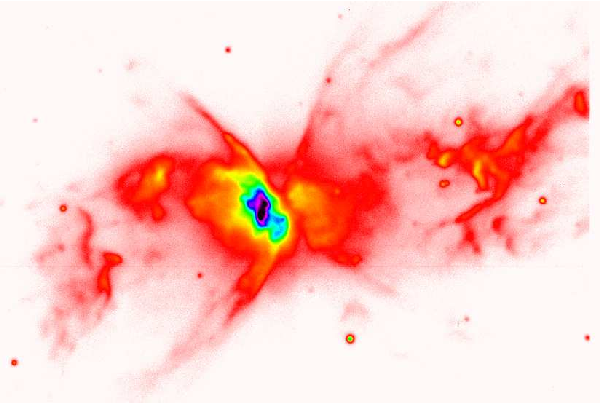
\includegraphics[width=!,height=\textheight]{./C/ngc6302_Rband.pdf}}
\vspace{5cm}
\begin{center}
  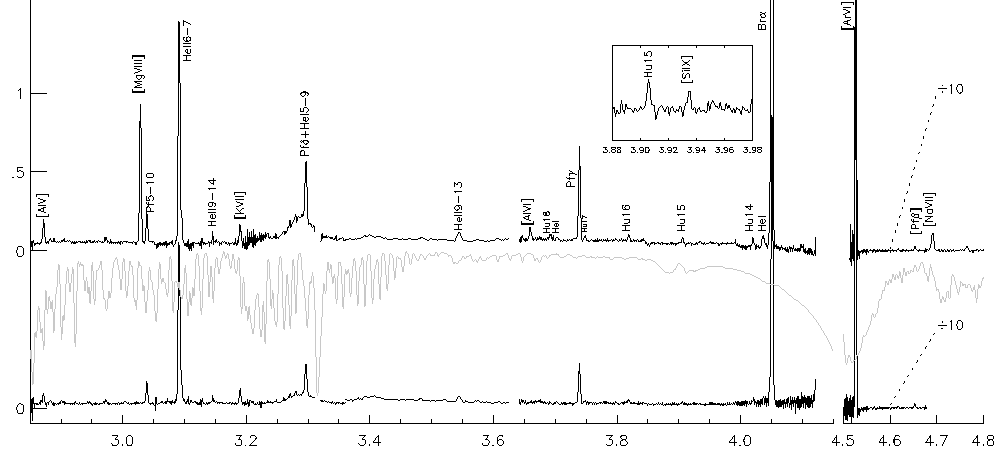
\includegraphics[width=25cm,height=!]{./C/specCGS4.pdf}
\end{center}

\foilhead{}

\vspace{4cm}
\begin{center}
  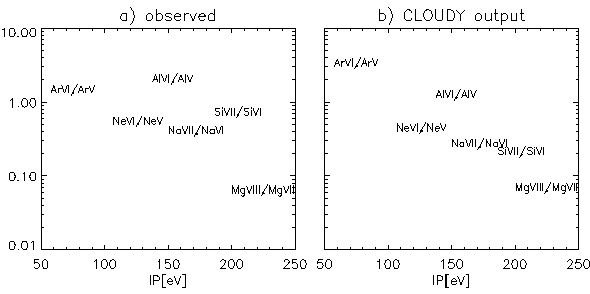
\includegraphics[width=25cm,height=!]{./C/ioncurve.pdf}
\end{center}

\foilhead{}

\vspace{10cm}
\begin{center}
  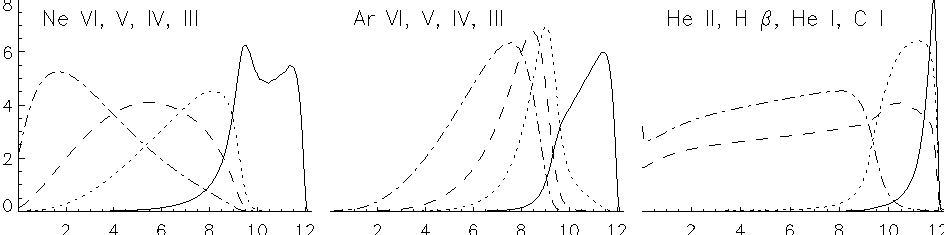
\includegraphics[width=25cm,height=!]{./C/struct_n6302.pdf}
\end{center}


\foilhead{}

\bgclear
Example input for  CLOUDY: {\tt parispn.in}\\

\medskip
\medskip
\medskip

{\tt black body, T=150,000K radius = 10\\
hden = 3.4771213\\
radius = 17\\
normalize to   Ca b  ~ 4861\\
abund he -1 C-3.523 N-4. O-3.222 ne-3.824 mg-4.523\\ 
}

\medskip

\textcolor{red}{Tarea}: Run the validation model for  CLOUDY 96 called
{\tt parispn.in}, and plot the relative abundances of each ionisation
stage for H, He and Ne. 

\foilhead{}

%\foilhead{\textcolor{red}{C$_4$} Modelos de nebulosas}

{$\bullet$ Str\"omgren Spheres}

{$\bullet$ Pure hydrogen nebulae}

(ver Problema 3-1 de Shu I)

{$\bullet$ Dusty H\,{\sc ii} regions.}

(Petrosian, Silk \& Field, 1972, ApJ, 177, 69; Spitzer)

{$\bullet$ Limits of the OTS approximation}.

see {\tt dhii.pdf}. 

\foilhead{3D codes}

Monte Carlo methods allow calculating the 3D photoionisation structure
given a proton density field. The best 3D code available is Mocassin
(Ercolano et al. 2003, MNRAS, 340, 1136). 
\begin{center}
  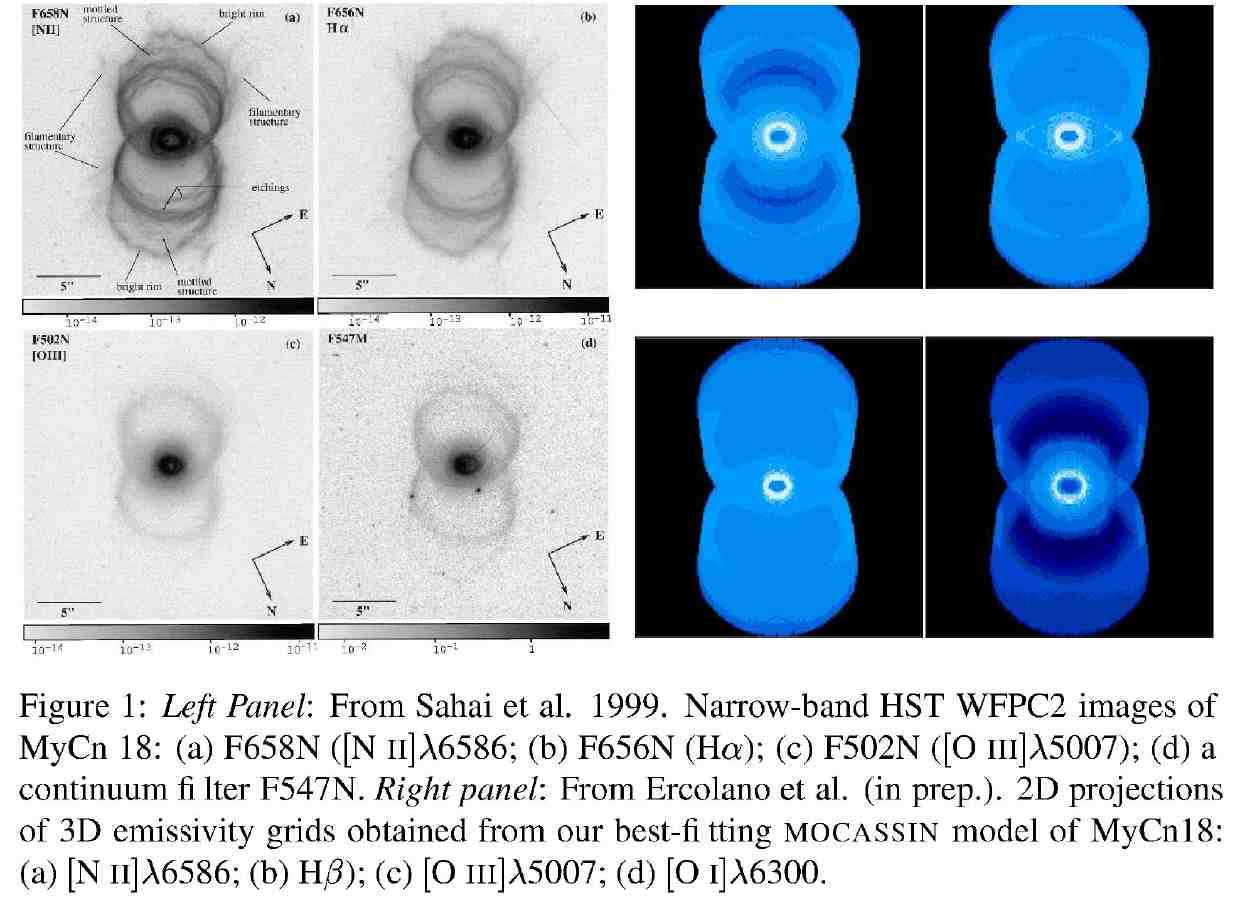
\includegraphics[width=0.7\textwidth,height=!]{./C/MyCn18_mocassin.jpg}
\end{center}


\foilhead{\textcolor{red}{C-\ref{item:diag}} Temperature
and density diagnostics}
\leftheader{C-\ref{item:diag}: Nebular diagnostics}

{$\bullet$ \bf Recombination lines of  H\,{\sc i}, He\,{\sc
ii}, and He\,{\sc i} } \\

The flux of a hydrogen recombination line in the optical is $F_{ij} =
\int ds d\Omega j_{ij}$, where the emissivity of a transition  $n_i
\leftarrow n_j$ populated by the recombination cascade is 
\[ 
j_{ij} = \frac{h \nu}{4 \pi} \sum_{L_i=0}^{n-1} \sum_{L_j=L_i\pm1} N_n
h\nu_{ij}.
\]
The occupation numbers $N_n$ can be calculated, and bear a weak
dependence on ${T_e,N_e}$. The radiative transfer effects are included
through an OTS approximation that distinguishes two cases (Baker \&
Menzel 1938, ApJ, 88, 52): case A, where the nebula is optically thin
in every transition (as well as in the Lyman continuum), and case B
where all photons from the Lyman serie, as well as the Lyman
continuum, are absorbed OTS, so that the effective fundamental state
in the recombination cascade is $n=2$.


\foilhead{Optical Recombination Lines - ORLs}

%\foilhead{\textcolor{red}{C$_5$} L\'{\i}neas de recombinaci\'on}

The effective recombination coefficient is defined through 
\[
N_p N_e \alpha_{ij}^\mathrm{eff} = \frac{4 \pi}{h \nu_{ij}}  j_{ij}.
\]
Hummer \& Storey (1987, MNRAS, 224, 801) give 
$\alpha_\mathrm{H\beta}^\mathrm{eff} =3.0~10^{-14}~$cm$^{-3}$, at
$10^4$~K (approximately  $\propto
\sqrt{1/T_e}$), and tabulate the emissivities of H\,{\sc i} and
He\,{\sc ii} recombination lines relative to $H_\beta$. The relative
emissivities for the He\,{\sc i} recombination lines are tabulated by
Smits, MNRAS, 251, 316. Those of O\,{\sc ii}, N\,{\sc ii}, N\,{\sc
iii}, Ne\,{\sc ii}, C\,{\sc ii} y C\,{\sc iii} have been computed by
Storey et al. and can be found in the recent literature.

Note that given $N_e$ and the flux of a recombination line, it is
straightforward to obtain the column of the corresponding ion. For
example the recombination spectrum of O\,{\sc ii} gives the column of
O$^{2+}$, which has the spectrum of O\,{\sc iii}.


\foilhead{Collisionally Excited Lines - CELs.}
\leftheader{C-\ref{item:diag}: Nebular diagnostics}


%\foilhead{\textcolor{red}{C$_5$} L\'{\i}neas excitadas por colisiones - CELs.}

The flux of an optically thin CEL $i \leftarrow j$ is given by
integrating the line emissivity along the optical path $s$:
\[
F_{ij} = \int ds \int d\nu \, d\Omega ~ j_\nu = \int ds \, d\Omega ~ \frac{b\,
A_{ij}\, h\nu_{ij}}{4\pi}~ N_j ,
\]
where  $N_j$ is the population of the excited level $j$, and where $b$
is the ``branching ratio'', in the general case where there is more
than one transition branching off the same upper level: $b = A_{ij} /
\sum_{k<j} A_{kj}$.

The principle underlying the diagnostic of physical conditions in
ionised nebulae is the dependence of $N_j(\vec{r})$ on
$T_e,N_e$. Neglecting radiative excitations (i.e. optically thin case),
\[
\sum_{i{\neq}j}
{n}_{j}{C}_{ji} +
\sum_{i<j}{n}_{j}{A}_{ji} = \sum_{i{\neq}j}{n}_{i}{C}_{ij}  + \sum_{i>j}{n}_{i}{A}_{ij}, 
\]
where $N_j = n_j \, N_\circ$, and $N_\circ$ is the ground state
population. In LS coupling the Hund rules give 2 to 5 levels in the
fundamental configuration of common ions. 

\foilhead{Temperature and density}

{$\bullet$} Density-sensitive pairs of  lines.  \\

%\begin{minipage}[t]{11cm}
%  \begin{center}
%    \includegraphics[width=10cm,height=!]{oii.pdf}
%  \end{center}
%\end{minipage}
%%\hfill
%\begin{minipage}[t]{15cm}

\begin{floatingfigure}{12cm}
\includegraphics[width=9cm,height=!]{./C/oii.pdf}
\end{floatingfigure}  \quad  The critical densities of both lines are 
 $N_c(\lambda3729) = 4\,10^{13}$cm$^{3}$ and $N_c(\lambda3726) =
2\,10^{4}$cm$^{-3}$, both comparable to typical nebular densities. The
ratio of these lines does not depend on the concentration of
O$^+$. Since the upper levels are very close in energy, their relative
populations are insensitive on temperature. The [O\,{\sc ii}] doublet
is a good diagnostic for densities close to the critical densities.

\foilhead{}

[O\,{\sc ii}] doublet for typical densities:
\begin{itemize}
\item $N_e \ll N_c$. \[ \frac{I(\lambda 3279)}{I(\lambda 3726)} =\frac{ N_e
N_1  \langle \sigma_{12} v \rangle \frac{h\nu_{21}}{4\pi}}{ N_e
N_1  \langle \sigma_{13} v \rangle \frac{h\nu_{31}}{4\pi}} = \frac{ \langle
\sigma_{12} v  \rangle}{\langle \sigma_{13} v  \rangle},\] independent
of $N_e$\footnote{and also of  $T_e$ because  $\sigma \propto g$ for
fine structure levels}
\item $N_e \gg N_c$. In this case  $N_3 = N_1 C_{13}/C_{31} = N_1 g_3
e^{-\chi_3/kT} / g_1 $  and 
\[\frac{I(\lambda 3279)}{I(\lambda 3726)} = \frac{A_{21}
N_2 g_2 }{A_{31}N_3 g_3}, \] independent of  $N_e$ and weakly
dependent on $T_e$.
\item In an intermediate case, we consider  $N_c(\lambda 3729) \ll N_c
\ll N_c(\lambda 3726)$:
\[\frac{I(\lambda 3279)}{I(\lambda 3726)} = \frac{g_2}{g_3}
\frac{A_{21}}{N_e \langle \sigma_{12} v \rangle} \propto
\sqrt{T_e}/N_e,\]  which is a function of  $N_e$.
\end{itemize}

%\end{minipage}



\foilhead{Temperature-sensitive pairs}

%\begin{minipage}[t]{8cm}
%  \begin{center}
%    \includegraphics[width=7cm,height=!]{oiii.pdf}
%  \end{center}
%\end{minipage}
%    \includegraphics[width=7cm,height=!]{oiii.pdf}
%\hfill
%\begin{minipage}[t]{15cm} 
%\vspace{-8cm}
\begin{floatingfigure}{8cm}
\includegraphics[width=7cm,height=!]{./C/oiii.pdf}
\end{floatingfigure}  These 3 transitions have $A \gtrsim 1$~s$^{-1}$,  $N_c \gg
10^{4}$~cm$^{-3}$, and $A_{32} \ll A_{31}$, so that 
\begin{eqnarray}
j(\lambda4363) & = &  N_e N_1 \langle \sigma_{13} v \rangle \frac{h \nu_{32}}{4\pi}, \nonumber \\
j(\lambda5007) & = &  N_e N_1 \left[ \langle \sigma_{12} v \rangle  +
\langle \sigma_{13} v \rangle  \frac{A_{32}}{A_{31}+A_{21}} \right] \frac{h \nu_{21}}{4\pi}, \nonumber 
\end{eqnarray}
where we have treated  $\lambda4959$ and $\lambda5007$ as a single
line. The ratio of these  {\bf two} lines is 
\[
\frac{I(\lambda 5007)}{I(\lambda4363)} = \frac{\lambda_{32}}{\lambda_{21}}
\left[1+\frac{\langle \sigma_{12} v \rangle}{\langle \sigma_{13} v
\rangle } \right].
\]
Remembering that  $\langle \sigma_{ij} v \rangle \propto T_e^{-1/2}
e^{-\chi_{ij}/kT_e}$, we see that the ratio $\frac{I(\lambda
5007)}{I(\lambda4363)} $ is sensitive on the temperature. One gets 
$\frac{I(\lambda 5007)}{I(\lambda4363)} \approx 8~\exp(33000/T_e)$.

%\end{minipage}



\foilhead{Density and the ORLs}


\begin{floatingfigure}{14cm}
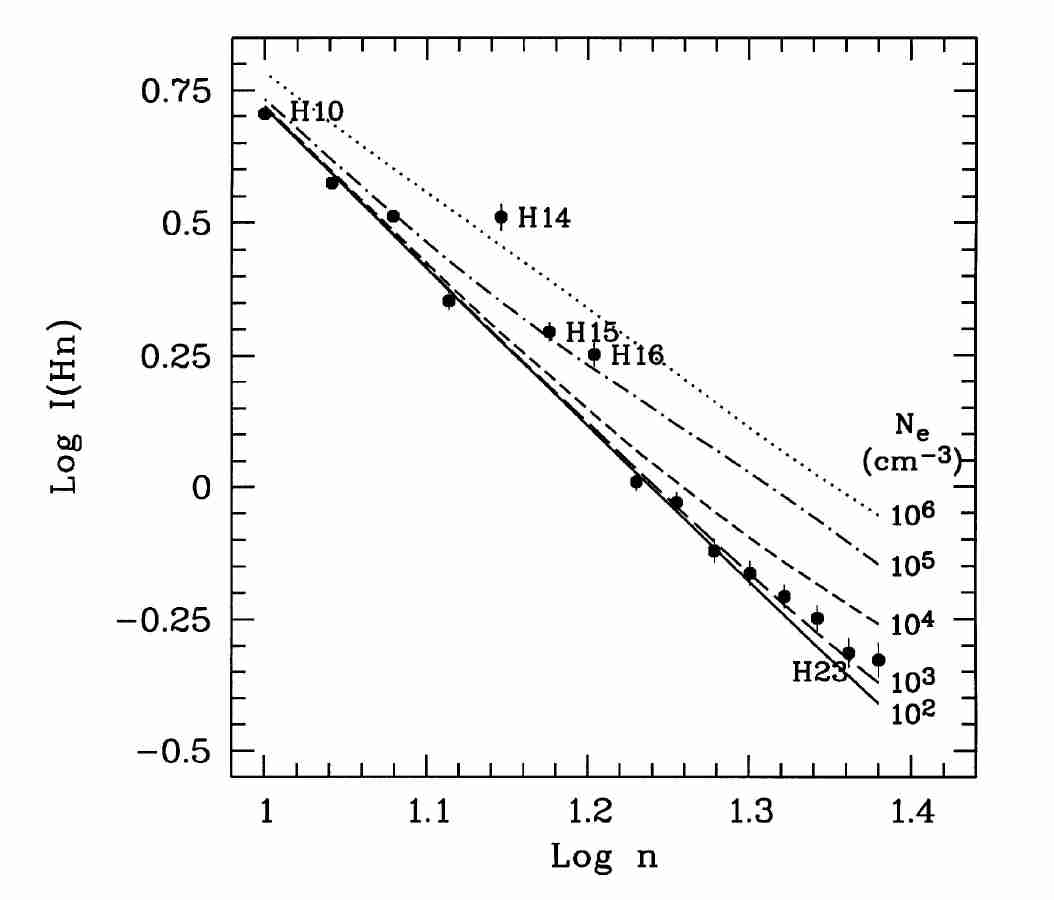
\includegraphics[width=13cm,height=!]{./C/Hn_Ne.jpg}
\end{floatingfigure}  The recombination lines have a very weak
dependence on density, which can be used as diagnostic (Liu et
al. 2000, MNRAS, 312, 585).

\foilhead{The line-continuum-temperature relationship}

The radio-continuum flux density of free-free radiation relates to the
H$\beta$ flux through
\[
F(H\beta) = 0.28 T_e^{-0.52} \nu^{0.1} F_\nu,
\]
which gives $T_e$. The recombination lines with $n\gg 1$ at radio
frequency are not extinct, and their emissivities can be calculated in
LTE (the correction is $\ll 1$ and is tabulated by Brocklehurst 1970,
MNRAS 148, 417).


\foilhead{Balmer and  Paschen discontinuity   }

\begin{minipage}[t]{13cm}
$BJ = \frac{I_c(\lambda3643)-I_c(\lambda3681)}{I(H11,\lambda3770)}.$
\\ $I_c(\lambda)$ is tabulated by Brown \& Mathews (1970, ApJ, 160,
939).

\begin{center}
  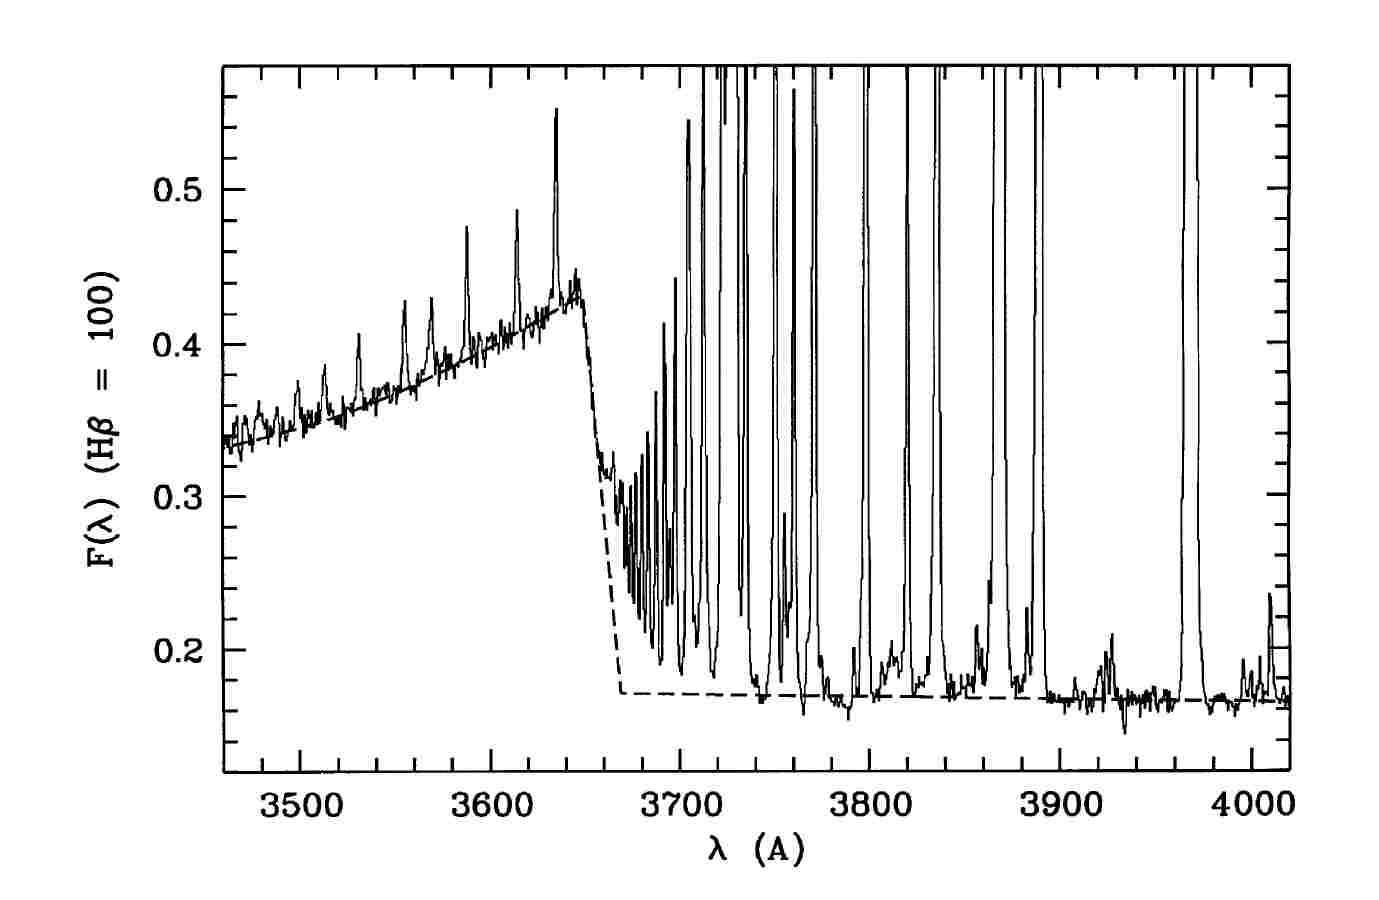
\includegraphics[width=12.5cm,height=!]{./C/bj_liu.jpg} \end{center}
\end{minipage}
\hfill
\begin{minipage}[t]{13cm}
He$^+$/H$^+$ = 0.1, He$^{++}$/H$^+$=0 (dots);
He$^+$/H$^+$ = He$^{++}$/H$^+$=0.05   (solid);
He$^+$/H$^+$ = 0, He$^{++}$/H$^+$=0.1   (dashed).
  \begin{center}
    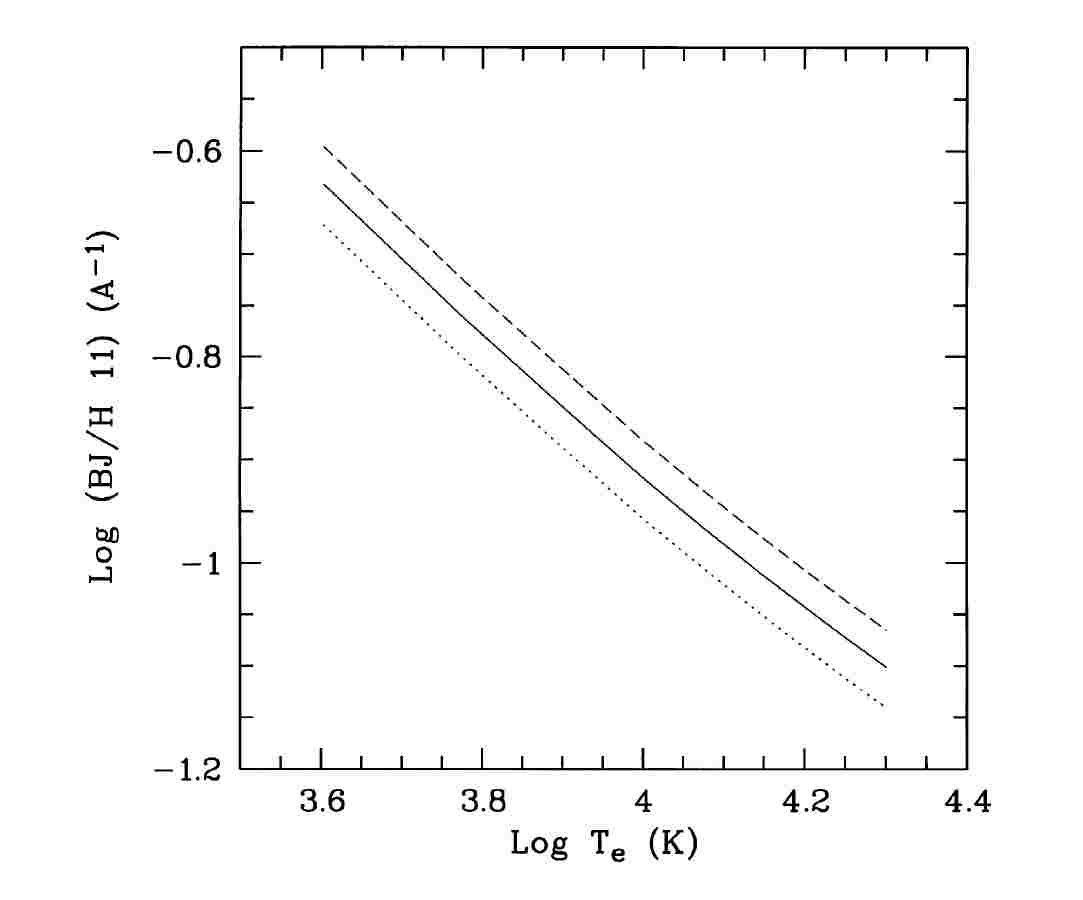
\includegraphics[width=12.5cm,height=!]{./C/BJ_T.jpg}
  \end{center}
\end{minipage}

The same analysis can be applied to the Paschen discontinuity at
8194\AA.

\foilhead{The ORL/CEL discrepancy }

\begin{center}
      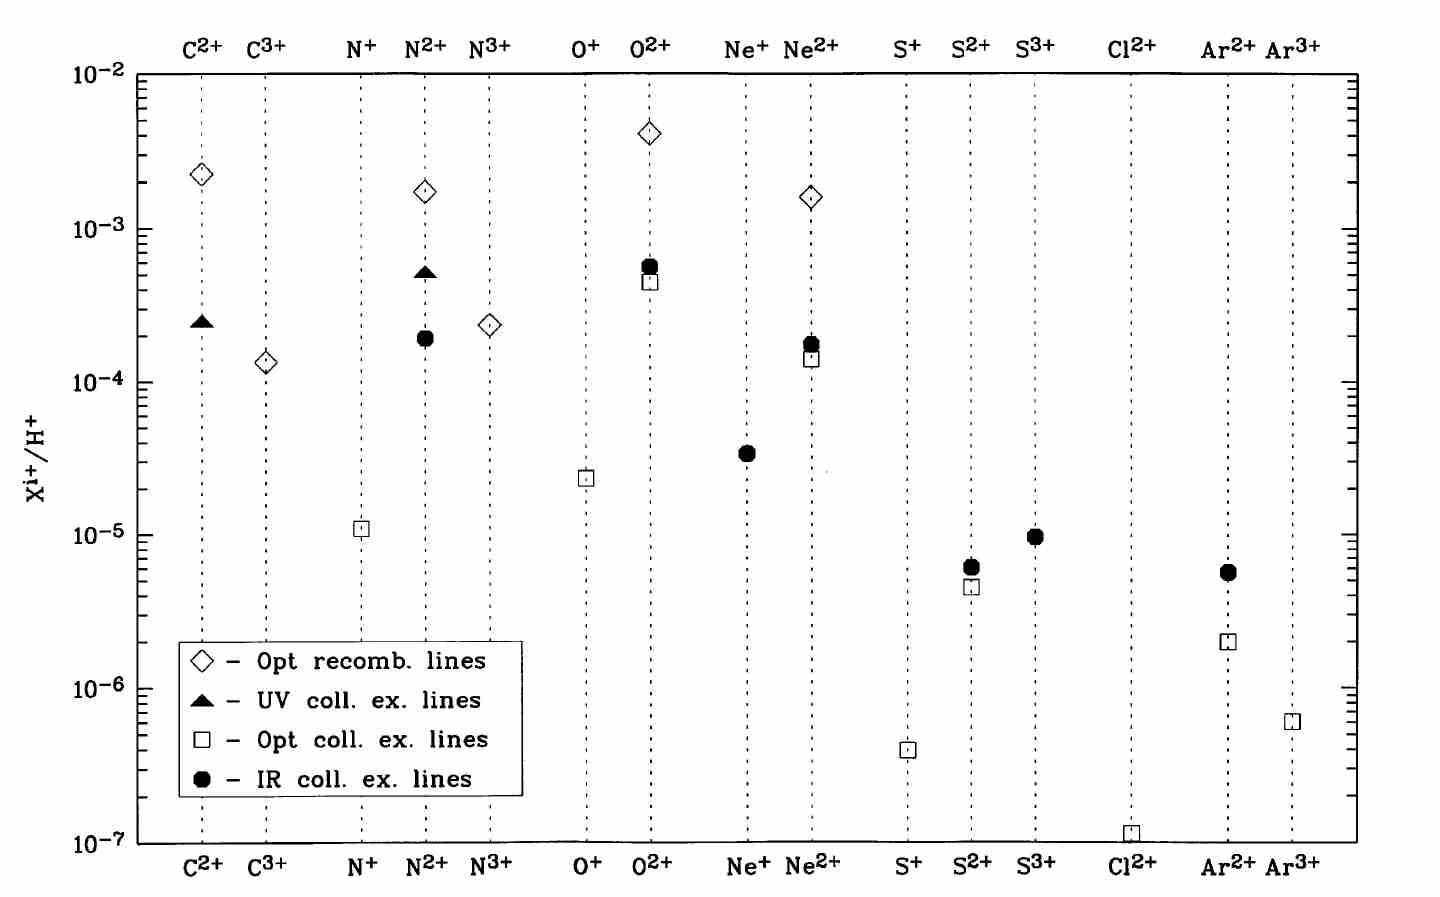
\includegraphics[width=0.9\textwidth,height=!]{./C/ORL_CEL_general.jpg}
\end{center}


\foilhead{ORL/CEL}

\begin{itemize}
\item In principle the best indicators of ionic abundances are the
ORLs, because the recombination coefficients of both hydrogen and
metals are approx. $\propto 1/\sqrt{T_e}$, so that the residual
dependence on temperature is very weak.

\item The difficulty with  ORLs is that their fluxes are  $10^{-3} -
10^{-4}$ weaker than H$\beta$.

\item By contrast the CELs have an exponential dependence on
temperature, and their fluxes are comparable to H$\beta$.

\end{itemize}

\foilhead{ORL/CEL}

\begin{center}
      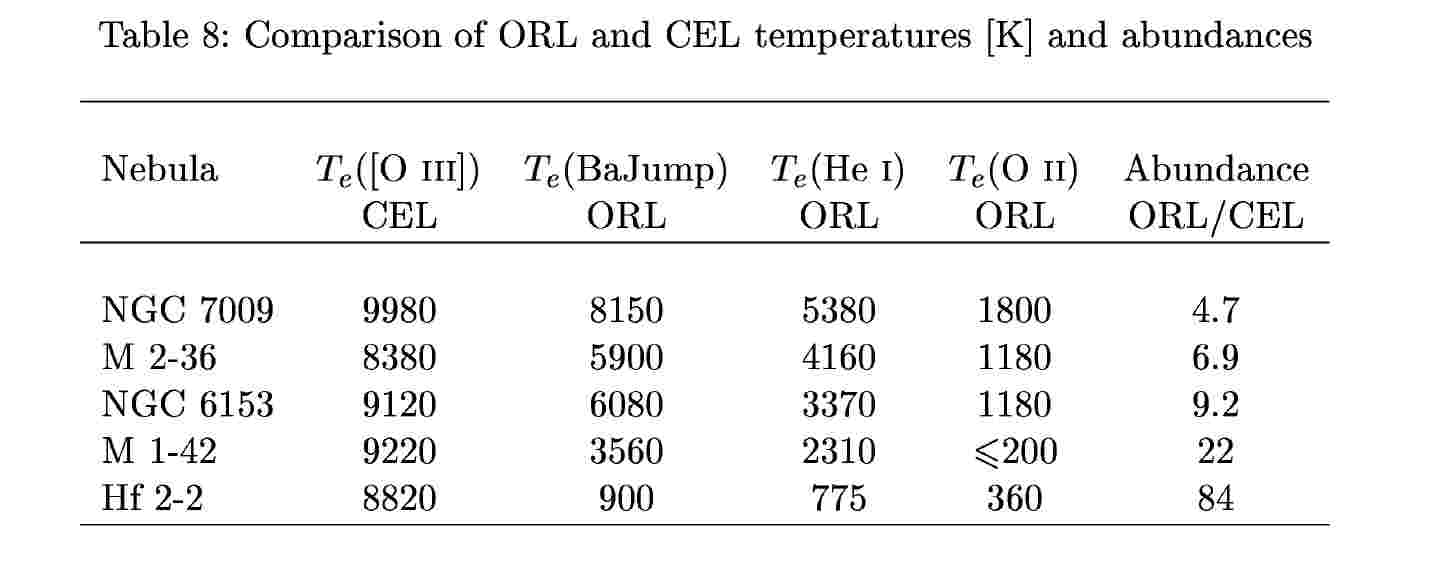
\includegraphics[width=\textwidth,height=!]{./C/orl_cel_table.jpg}
\end{center}

There is a systematic discrepancy between CELs and ORLs:\begin{itemize}
\item $T_e(\mathrm{CEL}) > T_e(\mathrm{ORL} \sim T_e(\mathrm{continuum})$
 
\item $N(X^{+i})(\mathrm{CEL}) < N(X^{+i})(\mathrm{ORL})$, although
the columns are similar when using the same temperatures.
\end{itemize}


\foilhead{\textcolor{red}{C$_5$} The ORL/CEL discrepancy  -
temperature fluctuations.  }

One strategy to reconcile the temperature discrepancy, original
proposed by Peimbert (1967, ApJ, 150, 825) to explain the systematic
discrepancy in $T($O\,{\sc iii}) and $T(\mathrm{continuum})$, is the
``$t^2$'' formalism. In this formalism one expands the CEL emissitivies
in small temperature fluctuations about a mean value:
\[
j(T) = j(T_\circ) + (T-T_\circ)
\left. \frac{dj}{dT}\right|_{T=T_\circ} + \left. \frac{1}{2} (T-T_\circ)^2
\frac{d^2j}{dT^2}\right|_{T=T_\circ}, \text{and integrating over  $ds$,}
\]
\[
\int N_e N_i j(T) ds = j(T_\circ) \int N_i N_e ds + \left. \frac{1}{2}
\frac{d^2j}{dT^2}\right|_{T=T_\circ} \int ds N_i N_e (T-T_\circ)^2,
\]
where the term of order 1 cancels out when choosing\[
T_\circ = \int ds N_i N_e T / \int ds N_i N_e \text{. ~~We define } 
t^2 = \frac{\int N_i N_e (T-T_\circ)^2 ds}{T_\circ^2  \int
ds N_i Ne }.\]

Two pairs of $T_e$-sensitive lines allow calculating $T_\circ$ and
$t^2$. In this formalism $T_\circ$ is {\bf the }  nebular temperature,
and is closer to the ORLs and to the continuum than to the CELs. In
other words $t^2$ effectively adopts the ORL values. 


\foilhead{ORL/CEL discrepancy - solution?}

An alternative to the $t^2$ formalism is to interpret the observed
discrepancies as real, and conclude there are cold and metal rich
inclusions in the nebulae. These inclusions may find their origin in
the evaporation of globules or ices on big-grains (or planetesimals)
for H\,{\sc ii} regions, or in the ejection of enriched stellar
material in the dredge-up of AGB precursors to planetary nebulae.


\begin{center}
      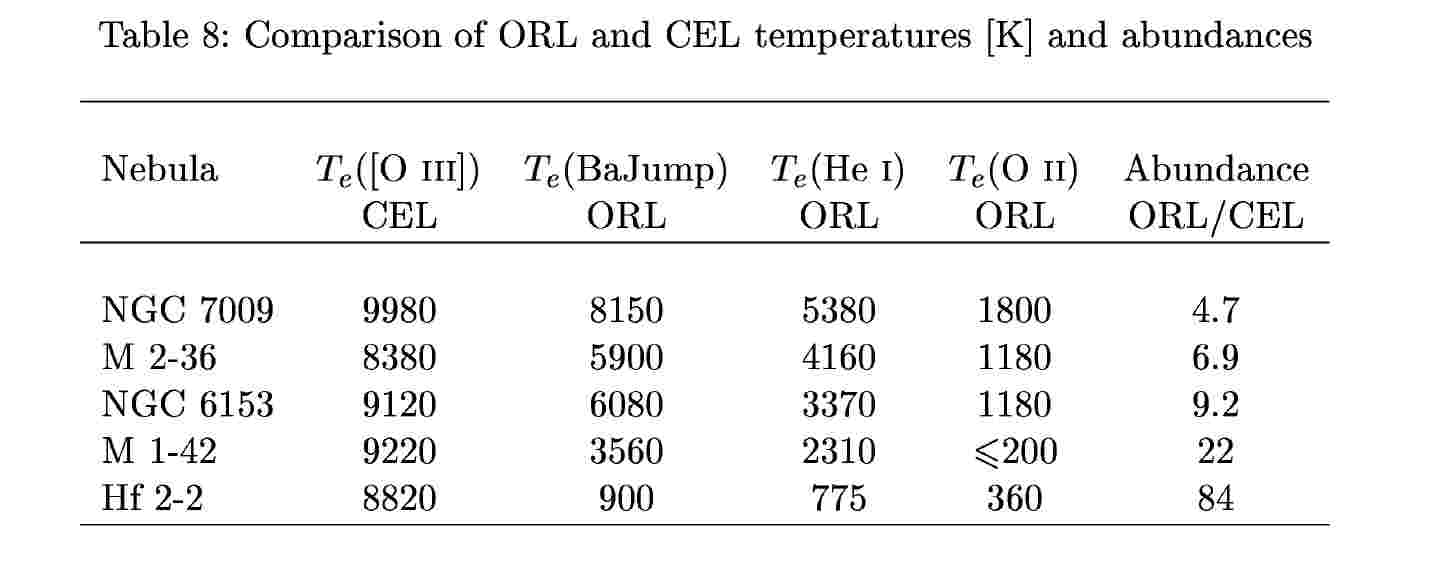
\includegraphics[width=\textwidth,height=!]{./C/orl_cel_table.jpg}
\end{center}

\foilhead{}
Photoionisation models with two phases indicate that the bulk of
nebular material should come from the `hot' component, which is traced
by the CELs (good news!). A test for this interpretation is to study
the thermal broadening of the ORLs, as observed by Barlow et
al. (astro-ph/0605235), who compared [O\,{\sc iii}]~4363\AA~ with the
sum of the O\,{\sc ii} ORLs at 4089\AA, 4275\AA~ and 4349\AA:
\begin{center}
      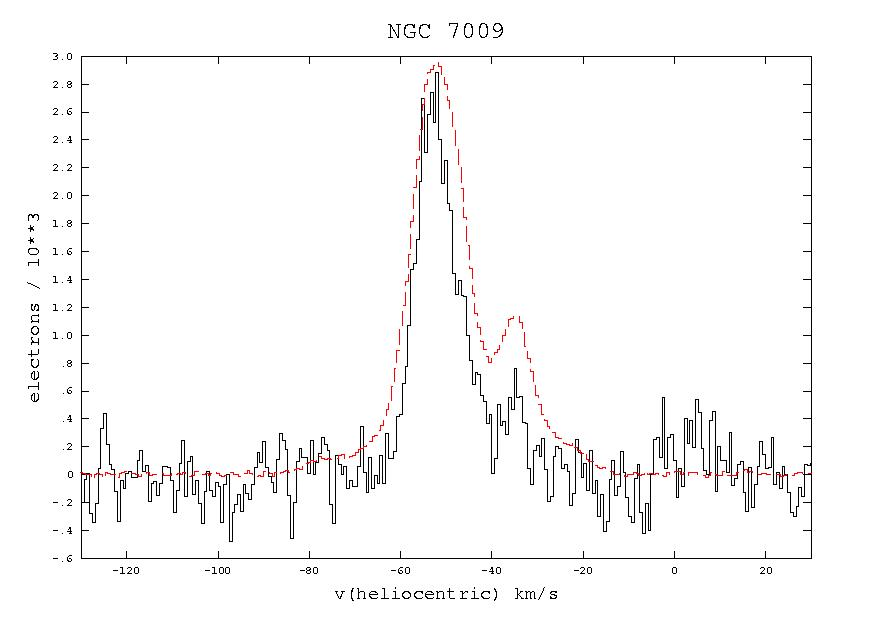
\includegraphics[width=0.7\textwidth,height=!]{./C/n7009_bHROS.jpg}
\end{center}


